
\documentclass[11pt]{isuthesis}
\usepackage[]{graphicx}\usepackage[]{color}
%% maxwidth is the original width if it is less than linewidth
%% otherwise use linewidth (to make sure the graphics do not exceed the margin)
\makeatletter
\def\maxwidth{ %
  \ifdim\Gin@nat@width>\linewidth
    \linewidth
  \else
    \Gin@nat@width
  \fi
}
\makeatother

\definecolor{fgcolor}{rgb}{0.345, 0.345, 0.345}
\newcommand{\hlnum}[1]{\textcolor[rgb]{0.686,0.059,0.569}{#1}}%
\newcommand{\hlstr}[1]{\textcolor[rgb]{0.192,0.494,0.8}{#1}}%
\newcommand{\hlcom}[1]{\textcolor[rgb]{0.678,0.584,0.686}{\textit{#1}}}%
\newcommand{\hlopt}[1]{\textcolor[rgb]{0,0,0}{#1}}%
\newcommand{\hlstd}[1]{\textcolor[rgb]{0.345,0.345,0.345}{#1}}%
\newcommand{\hlkwa}[1]{\textcolor[rgb]{0.161,0.373,0.58}{\textbf{#1}}}%
\newcommand{\hlkwb}[1]{\textcolor[rgb]{0.69,0.353,0.396}{#1}}%
\newcommand{\hlkwc}[1]{\textcolor[rgb]{0.333,0.667,0.333}{#1}}%
\newcommand{\hlkwd}[1]{\textcolor[rgb]{0.737,0.353,0.396}{\textbf{#1}}}%

\usepackage{framed}
\makeatletter
\newenvironment{kframe}{%
 \def\at@end@of@kframe{}%
 \ifinner\ifhmode%
  \def\at@end@of@kframe{\end{minipage}}%
  \begin{minipage}{\columnwidth}%
 \fi\fi%
 \def\FrameCommand##1{\hskip\@totalleftmargin \hskip-\fboxsep
 \colorbox{shadecolor}{##1}\hskip-\fboxsep
     % There is no \\@totalrightmargin, so:
     \hskip-\linewidth \hskip-\@totalleftmargin \hskip\columnwidth}%
 \MakeFramed {\advance\hsize-\width
   \@totalleftmargin\z@ \linewidth\hsize
   \@setminipage}}%
 {\par\unskip\endMakeFramed%
 \at@end@of@kframe}
\makeatother

\definecolor{shadecolor}{rgb}{.97, .97, .97}
\definecolor{messagecolor}{rgb}{0, 0, 0}
\definecolor{warningcolor}{rgb}{1, 0, 1}
\definecolor{errorcolor}{rgb}{1, 0, 0}
\newenvironment{knitrout}{}{} % an empty environment to be redefined in TeX

\usepackage{alltt}
\newcommand{\SweaveOpts}[1]{}  % do not interfere with LaTeX
\newcommand{\SweaveInput}[1]{} % because they are not real TeX commands
\newcommand{\Sexpr}[1]{}       % will only be parsed by R


\usepackage{graphicx}
%---------------------------------------------------
\usepackage{color}
\usepackage[dvipsnames,svgnames]{xcolor}
\usepackage{wrapfig,float}
\usepackage{caption}
\usepackage{subcaption}
\usepackage{graphicx}
\usepackage{amssymb}
\usepackage{amsmath}
\usepackage{url}
\usepackage{ulem}
\usepackage[section]{placeins}
\usepackage{sidecap}
\usepackage{multirow}
\usepackage{bbm}
\usepackage[colorinlistoftodos]{todonotes}
%---------------------------------------------------

% Standard, old-style thesis
\usepackage{isutraditional}   \chaptertitle
% Old-style, thesis numbering down to subsubsection
\alternate
\usepackage{rotating}
% Bibliography without numbers or labels
\usepackage{natbib}
\bibliographystyle{apa}
%\includeonly{titletoc,chapter1}
%Optional Package to add PDF bookmarks and hypertext links
\usepackage[pdftex,hypertexnames=false,linktocpage=true]{hyperref}
\hypersetup{colorlinks=true,linkcolor=blue,anchorcolor=blue,citecolor=blue,filecolor=blue,urlcolor=blue,bookmarksnumbered=true,pdfview=FitB}

%---------------------------------------------------




\begin{document}

\graphicspath{{Figure/LitReview/}{Images/LitReview/}}
\renewcommand{\floatpagefraction}{.99}





% Chapter 1 of the Thesis Template File
\chapter{OVERVIEW}

\section{Goals of Statistical Graphics}

\section{Designing graphics for the human perceptual system}
\subsection{The Human Visual System}
Basic overview of structure, to serve as a reference

In order to design graphics for the human perceptual system, we must understand, at a basic level, the makeup of the perceptual system. There are multiple levels of perception that must correctly function in order to perceive visual stimuli successfully, but a somewhat simplistic higher-level analogy would be that we must understand both the hardware and software of the human visual system to create effective graphics.
The ``hardware", in this analogy, consists of the neurons that make up the eyes, optic nerve, and the brain itself. The higher-level functions (object recognition, working memory, etc.) comprise the ``software" component. In addition, much like computer software, there are different programs running simultaneously; these programs may interact with each other, run sequentially, or run in parallel. The following sections provide an overview of the grey-matter (hardware) components of the visual system as well as the higher-level cognitive heuristics (software) that order the raw input and construct our visual environment. 

\subsubsection{Hardware}
The physiology of perception is complex; what follows is a high-level overview of the physiology of perception, focusing on the areas most important to the perception of statistical graphics. This physiological information is important in understanding the difference between the sensation (i.e. the retinal image) and the perception (the corresponding mental representation), which is an important distinction in understanding how statistical graphics are perceived. 

\paragraph{The Eye}
The receptors which translate wavelengths of light into neural impulses are located in the retina, at the back of the eye. These receptors are specialized neurons, known as rods and cones, which perceive light intensity and wavelength, respectively. One section of the retina, known as the fovea, contains only cones; the rest of the retina contains a mixture of rods and cones. These rods and cones are responsible for translating the information contained in visual-spectrum electromagnetic waves into neural signals. Figure \ref{fig:retina} depicts the structure of the eye with a closeup of the retina. Disorders which affect these receptor cells, such as color blindness, can affect how those affected perceive statistical graphics. 

Figure \ref{fig:ColorRange} shows the responsiveness of rods and each of the three types of cones to wavelengths of light in the visual spectrum. 

\begin{figure}
\centering
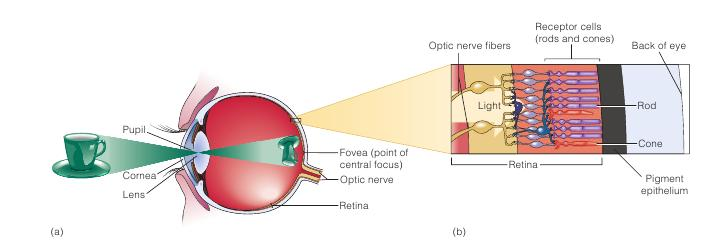
\includegraphics[width=.8\textwidth, keepaspectratio=TRUE]{Figure/LitReview/Retina}
\caption[The human eye, with closeup of receptor cells in the retina]{The human eye, with closeup of receptor cells in the retina. Image from \protect\citealt{goldstein}, chapter 3} \label{fig:retina}
\end{figure}

\begin{figure}
\centering
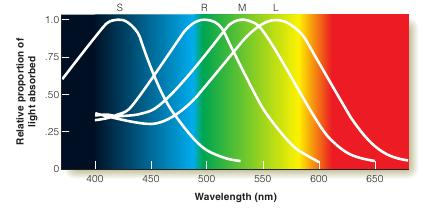
\includegraphics[width=.8\textwidth, keepaspectratio=TRUE]{Figure/LitReview/AbsorptionSpectra}
\caption[Absorption spectra of retinal cells]{Absorption spectra of rods and short, medium, and long wave cones.} \label{fig:retina}
\end{figure}

\begin{itemize}
\item Specific biology of the visual system - retina, optic nerve, cortex, etc. 

\item Difference between ``sensation" and ``perception"

\item Motion? (for interactive graphics)
\end{itemize}

\subsubsection{Software}
\begin{itemize}
\item Attention and perception

\item parallel processing - HCI handbook picture: summary of graphical perception

\item gestalt movement - wholistic approach

\item stored ``gist" and cognitive psych

\item Mention color choice (Light (2005) article) and prevalence of colorblindness. Logarithmic perception (Sun \& Varshney) and Weber-Fechner. 
\end{itemize}

\subsubsection{Bugs}
\begin{itemize}
\item Optical Illusions - Accounting for perceptual oddities that are inherent in the visual system, how to avoid triggering those heuristics. Hermann grid, cafe wall, ponzo illusion
\item Colorblindness
\item 
\end{itemize}


\section{Statistical Graphics}
\begin{itemize}
\item Cleveland \& McGill
\item Healey
\item Heuristic guidelines i.e. Kosslyn and Tufte
\item Grammar of graphics allows us to test graphics which display the same information in different ways for comparable accuracy
\end{itemize}
Emphasize the low-level stuff vs. the higher-level stuff that focuses on preattentive information (i.e. not what we care about) and the gap in the middle where graphics are tested in more practical scenarios.

\subsection{Optical illusions and statistical graphics}
three-dimensional context, other ways to trigger optical illusions with graphics. Importance of being aware of the heuristics the brain uses so that problematic graphics can be avoided. 

\subsection{Interactive graphics?} 
Not sure if this should be a subsection, but graphics that respond to human interaction violate the two-dimensional graphic paradigm somewhat, which means there are a whole 'nother set of issues to consider... motion illusions, grouping, etc.

\section{Testing Statistical Graphics}
Methodology for testing graphical perception in humans. Talk about masking, the power of suggestion, habituation, etc. as well as paradigms - search and find, response time, numerical judgments, signal detection, eye tracking. 
\begin{itemize}
  \item Tukey
  \item Cleveland \& McGill
  \item Lineups
\end{itemize}

\end{document}
